% !TEX root = ../MasterThesis_Onoe.tex
% 上記はただのコメントではなく親ファイルの場所を教えているので
% 消してしまうとファイルごとのタイプセットができなくなるので注意。
% 親ファイル名を変更したときはここも変更する。

\appendix 

\chapter{AppendixA} \label{sec:Appendix}
\section{飛跡のパラメータ}
\subsection{LDC座標系}
ILCにおいて検出器を通過する荷電粒子には、飛跡を記述する際に専用の手法が用いられており、それによってシミュレーションツールなどで変換を行うことなく、データを解析することができる。この手法はILDの母体となったLarge Detector Concept (LDC) よって定義された座標系\cite{ldc}を基に定義されており、LDC座標系は次のように定義される。
\begin{enumerate}
\item 右手系直交座標。
\item 電子陽電子の相互作用点を原点とする。
\item ビーム方向に沿ってz軸をとる。
\item 垂直上方向にy軸をとる。
\end{enumerate}

この座標系における任意のベクトル$\bm{v}$は球面座標系において、次のように表される。

\begin{align}
\mathbf{v} &= \left(
\begin{array}{c}
|\mathbf{v}| \sin \theta \cos \phi \\
|\mathbf{v}| \sin \theta \sin \phi \\
|\mathbf{v}| \cos \theta \\
\end{array}
\right) \\
\nonumber \theta& \in [0,\pi ] \\
\nonumber \phi &\in [-\pi , \pi ]
\end{align}

\subsection{飛跡パラメータ}
ILCで発生する荷電粒子は一定の磁場の影響を受け、螺旋軌道を描く。磁場はz軸に並行な方向に一様にかかるものとする。この時、荷電粒子の飛跡はxy平面への射影における円となり、z軸方向の変位は弧の長さsの線形関数となる。

荷電粒子は運動の基準点$\mathbf{P}^r = \left( P_x^r, P_y^r, P_z^r \right)$と飛跡パラメータ$\left( \Omega, {\phi}_0, d_0, z_0, \tan \lambda \right)$によって定義される。また、以下の定義において$\mathbf{P}^0$はxy平面上の基準点への最近接点を表す。
\subsubsection{xy平面}
xy平面では荷電粒子の移動は、以下のように定義される。\cite{lcio}
\begin{itemize}
\item ${\phi}_0$は運動量の$P_0$における方位角を表す。\\
\item $\Omega$は飛跡の曲率を表す。\\
\begin{align}
|\Omega | = \frac{1}{R}
\end{align}
ここで、Rは飛跡の曲率半径を表す。\\
\item $d_0$はxy平面のインパクトパラメータを表す。$\mathbf{d} = (d_x, d_y)$を任意の点$\mathbf{P}^r$から$\mathbf{P}^0$までのベクトルとする。\\
\begin{align}
\mathbf{d} = \mathbf{P}^0 - \mathbf{P}^r
\end{align}
また、$\mathbf{P}^0$から飛跡への法線ベクトルを$\mathbf{n}_{pca}$とすると、$d_0$は以下のように表される。
\begin{align}
d_0 = \mathbf{n}_{pca} \cdot \mathbf{d} = - ( P_x^r - P_x^0 ) \sin {\phi}_0 +  ( P_y^r - P_y^0 ) \cos {\phi}_0
\end{align}
$|\mathbf{n}_{pca}|$であるため、$|d_0|$はxy平面における$\mathbf{P}^r$と$\mathbf{P}^0$の距離を表す。
\end{itemize}
xy平面における円の中心点$\mathbf{P}^c$は、通常$\mathbf{P}^r$と異なる点を取ることが多く、軌道上の任意の点における運動量を$\mathbf{P} = \left( P_x, P_y, P_z \right)$とすると、$\mathbf{P}^c$は以下のように計算される。
\begin{align}
P_x^c &= P_x + \frac{\sin \phi}{\Omega}\\
P_y^c &= P_y + \frac{\cos \phi}{\Omega}\\
\end{align}
\begin{figure}[H]
	\begin{center}
 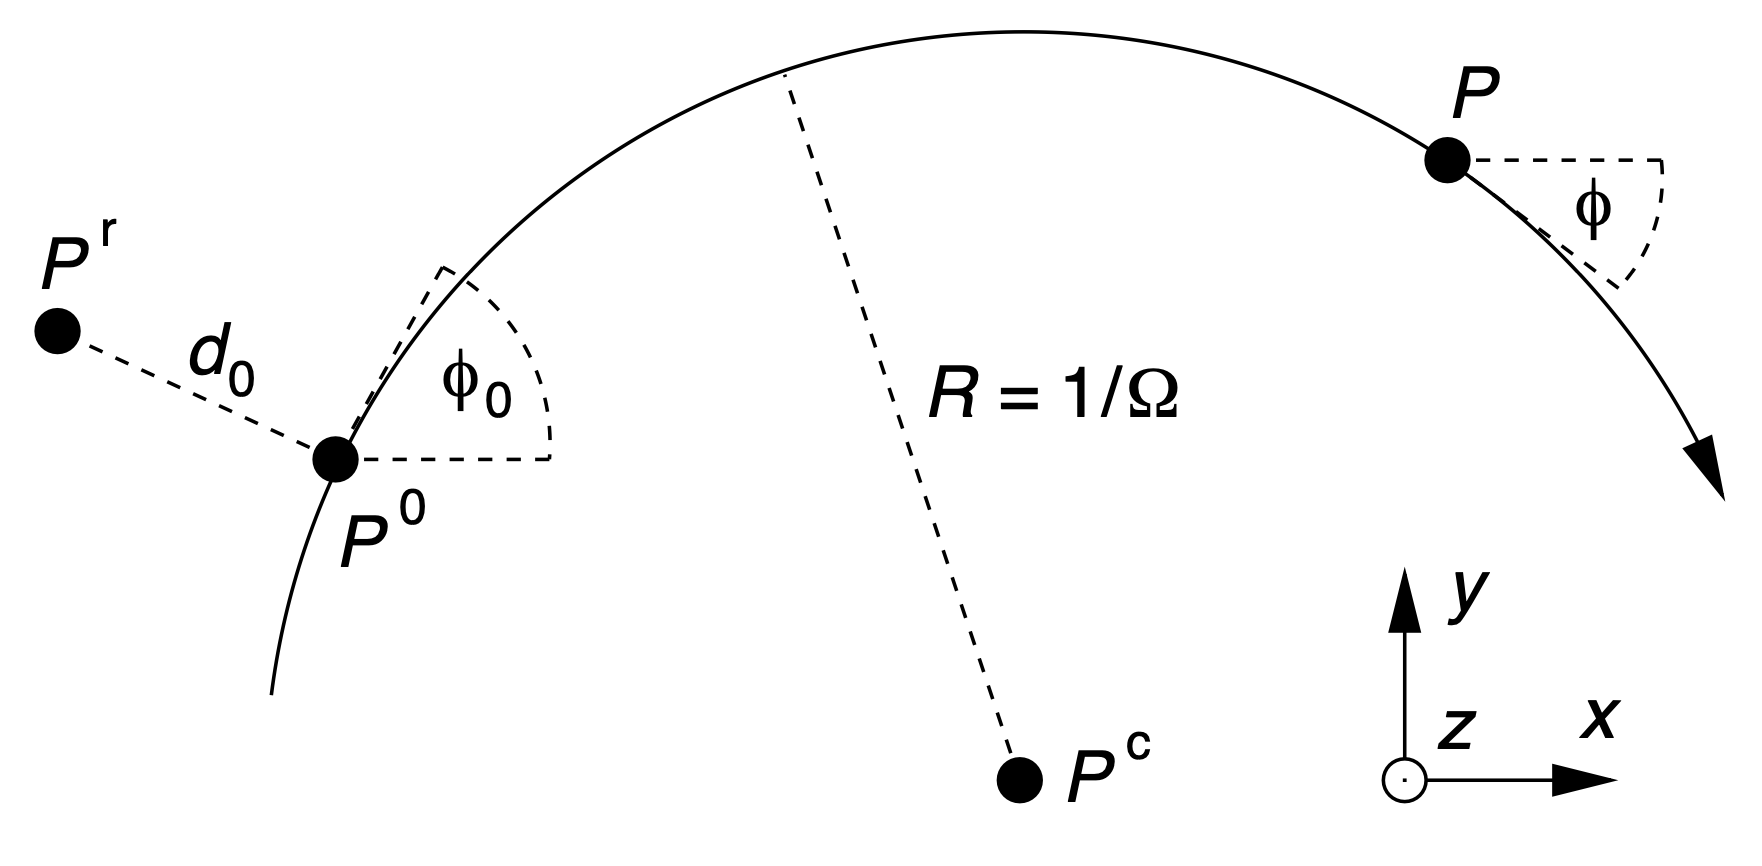
\includegraphics[keepaspectratio, scale=0.4]
 	{Figure/Appendix/xy.png}
 		\caption{飛跡の螺旋軌道をxy平面へ射影した図。軌道は中心点$\mathbf{P}^c$、半径Rをもつ円弧で表される。また、全ての飛跡パラメータは基準点$\mathbf{P}^r$を中心に与えられる。}
 		\label{xy}
	\end{center}
\end{figure}

\subsubsection{sz平面}
sz平面において、飛跡は直線に沿って移動し、2つのパラメータ$(\tan \lambda, z_0)$によって表される。
\begin{itemize}
\item $\tan \lambda$はsz平面における直線の傾き$dz/ds$を表し、運動量ベクトル $\mathbf{p} = \left( p_x, p_y, p_z \right)$に対して以下のように計算される。
\begin{align}
\tan \lambda =\frac{p_z}{\sqrt{p_x^2 + p_y^2}} = \cot \theta
\end{align}
\item $z_0$は基準点$\mathbf{P}^r$から$\mathbf{P}^0$までのz軸上の距離を表す。\\
\begin{align}
z_0 = P_z^0 - P_z^r
\end{align}
\end{itemize}
これらを踏まえ、飛跡のsz平面射影の軌跡zは、xy平面における飛跡の経路積分sを用いて次のように表される。
\begin{align}
z = ( z_0 + P_z^r) + s \cdot \tan \lambda
\end{align}
\begin{figure}[H]
	\begin{center}
 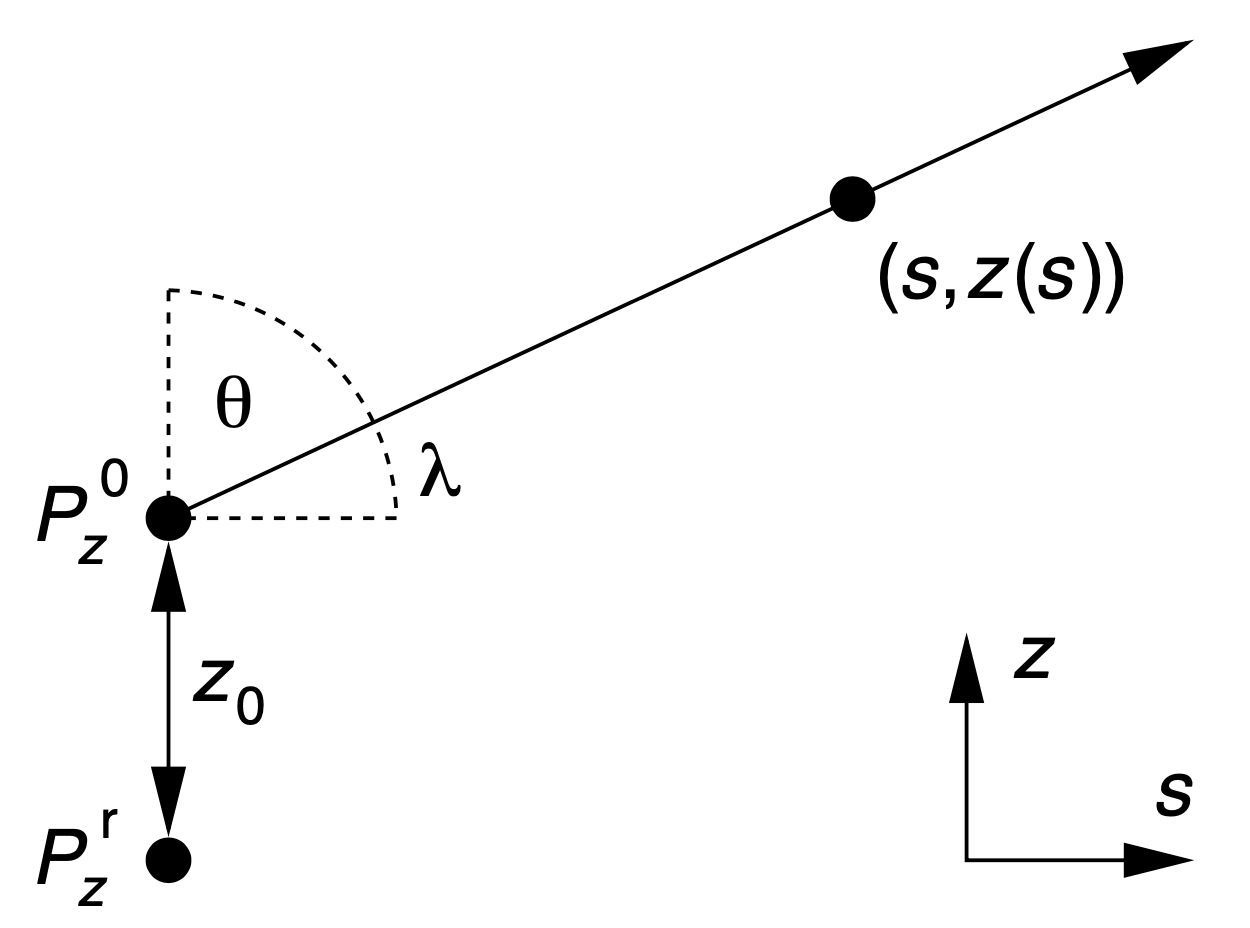
\includegraphics[keepaspectratio, scale=0.4]
 	{Figure/Appendix/sz.png}
 		\caption{sz平面}
 		\label{sz}
	\end{center}
\end{figure}
